\documentclass[11pt]{article}
\usepackage[letterpaper,margin=0.9in,headheight=14pt]{geometry}
\usepackage[T1]{fontenc}
\usepackage{lmodern}
\usepackage{microtype}
\usepackage{amsmath,amssymb,amsthm,mathtools}
\usepackage{enumitem}
\usepackage{booktabs,array,longtable,tabularx}
\usepackage{xcolor}
\usepackage{fancyhdr}
\usepackage[hidelinks]{hyperref}
\usepackage{listings}
\usepackage{tikz}
\usetikzlibrary{arrows.meta,positioning,shapes.geometric,fit}

\hypersetup{
  pdftitle={Automated Logical Deciders: Certificate-Indexed Halting, Multiagent Search, Provenance-Aware Shared Lemma Pools, and ML Guidance},
  pdfauthor={Brian Tenneson},
  pdfsubject={A rigorous theory of certificate-indexed multiagent automated logical deciders},
  pdfkeywords={automated logical decider, automated theorem proving, independence, certificate, halting, multiagent, lemma pool, machine learning}
}

\definecolor{deepblue}{RGB}{24,55,104}
\definecolor{softblue}{RGB}{232,239,249}
\definecolor{softgray}{RGB}{245,245,245}
\definecolor{darkgreen}{RGB}{31,92,66}
\definecolor{darkred}{RGB}{130,35,35}

\newtheorem{theorem}{Theorem}[section]
\newtheorem{proposition}[theorem]{Proposition}
\newtheorem{corollary}[theorem]{Corollary}
\newtheorem{lemma}[theorem]{Lemma}
\theoremstyle{definition}
\newtheorem{definition}[theorem]{Definition}
\newtheorem{example}[theorem]{Example}
\newtheorem{protocol}[theorem]{Protocol}
\theoremstyle{remark}
\newtheorem{remark}[theorem]{Remark}
\newtheorem{conjecture}[theorem]{Conjecture}

\newcommand{\N}{\mathbb N}
\newcommand{\Np}{\mathbb N_{+}}
\newcommand{\Pow}{\mathcal P}
\newcommand{\Con}{\operatorname{Con}}
\newcommand{\Mod}{\operatorname{Mod}}
\newcommand{\Cert}{\operatorname{Cert}}
\newcommand{\Ver}{\operatorname{Ver}}
\newcommand{\Len}{\operatorname{len}}
\newcommand{\Pool}{\mathcal L}
\newcommand{\MetaPool}{\mathcal K}
\newcommand{\Ev}{\mathcal E}
\newcommand{\Status}{\operatorname{Status}}
\newcommand{\Unknown}{\mathsf{UNKNOWN}}
\newcommand{\Der}{\mathsf{DERIVABLE}}
\newcommand{\Refut}{\mathsf{REFUTABLE}}
\newcommand{\Both}{\mathsf{BOTH}}
\newcommand{\Ind}{\mathsf{INDEPENDENT}}
\newcommand{\Inc}{\mathsf{INCONSISTENT}}
\newcommand{\NPlus}{\mathsf{N}_{+}}
\newcommand{\NMinus}{\mathsf{N}_{-}}
\newcommand{\Cons}{\operatorname{Cons}}
\newcommand{\Supp}{\operatorname{supp}}
\newcommand{\Plus}{\mathsf{P}}
\newcommand{\Minus}{\mathsf{N}}
\newcommand{\BotEv}{\mathsf{B}}
\newcommand{\IndEv}{\mathsf{I}}
\newcommand{\ALD}{\mathsf{ALD}}
\newcommand{\ATP}{\mathsf{ATP}}
\newcommand{\M}{\mathcal M}
\newcommand{\T}{\mathcal T}
\newcommand{\F}{\mathcal F}
\newcommand{\Gammaa}{\Gamma}
\newcommand{\negc}{\neg c}
\newcommand{\bottomf}{\bot}

\pagestyle{fancy}
\fancyhf{}
\lhead{Automated Logical Deciders}
\rhead{Tenneson, Research Supplement}
\cfoot{\thepage}
\renewcommand{\headrulewidth}{0.4pt}

\setlist[itemize]{leftmargin=1.5em}
\setlist[enumerate]{leftmargin=2em}
\setlength{\parskip}{0.35em}
\setlength{\parindent}{0pt}

\lstset{
  basicstyle=\ttfamily\small,
  backgroundcolor=\color{softgray},
  frame=single,
  breaklines=true,
  columns=fullflexible,
  keepspaces=true
}

\begin{document}

\hypersetup{pageanchor=false}
\begin{titlepage}
\thispagestyle{empty}
\centering
\vspace*{0.45in}
{\Huge\bfseries Automated Logical Deciders\par}
\vspace{0.18in}
{\LARGE\bfseries Certificate-Indexed Halting, Multiagent Search,\\
Provenance-Aware Shared Lemma Pools, and Machine-Learned Guidance\par}
\vspace{0.38in}
{\Large A rigorous research supplement in the spirit of\\
\emph{Depths of Induction, ML-Guided Proof Search, and Formalized Self-Awareness}, Version 47\par}
\vspace{0.55in}
{\Large Brian Tenneson\par}
\vspace{0.07in}
{\large M.S., Applied Data Science\par}
{\large Currently Unaffiliated\par}
\vfill
{\large August 2, 2026\par}
\vspace{0.28in}
\begin{minipage}{0.86\textwidth}
\small
This supplement develops Automated Logical Deciders (ALDs) as certificate-producing, multiagent proof-search systems. Four principal roles search in parallel for a proof of a conjecture, a proof of its negation, a contradiction, and metatheoretic certificates that each side is underivable. Every agent can read from and propose additions to a shared lemma pool in every round. Pool entries are independently verified, typed by object or metatheory, and labeled by the assumptions on which they depend. The central principle is that operational termination, exhaustive closure, and logical settlement are distinct. A conclusive status is licensed only by a status-appropriate certificate.
\end{minipage}
\vspace{0.34in}

{\small Copyright \textcopyright\ 2026 Brian Tenneson. All Rights Reserved.\par}
\end{titlepage}
\hypersetup{pageanchor=true}

\pagenumbering{roman}
\section*{Abstract}
\addcontentsline{toc}{section}{Abstract}
An ordinary target-search automated theorem prover is naturally success-oriented: it halts when it finds a proof. That architecture cannot detect independence merely by running a prover for a conjecture and another for its negation, because when both conjectures are underivable both searches may run forever. This paper replaces failure-to-halt with positive, independently checkable certificates of nonderivability. It defines a multiagent Automated Logical Decider with four principal roles: a proponent for $c$, an opponent for $\neg c$, an inconsistency agent for $\bot$ or $c\wedge\neg c$, and an independence agent searching in a declared metatheory for two nonderivability certificates. All agents can read from and contribute to a provenance-aware shared lemma pool in every round; only verifier-accepted entries are published, and every entry records the assumptions under which it is valid. Sufficient certificates include finite exhaustive saturation, preserved invariants, model pairs, relative-consistency arguments, and arbitrary checked metaproofs. The paper proves soundness, context-safe and conservative lemma reuse, certificate-horizon results, fair multiagent halting under certificate coverage, a no-false-independence theorem for timeouts, and undecidability barriers to total ALDs. It then adds machine learning as a soundness-neutral policy for ranking actions, allocating resources, and selecting reusable lemmas, provided independent verification and a fairness-preserving exploration component remain fixed. A literature comparison concludes that the ingredients have substantial prior art---including the TPTP SZS \emph{NoConsequence} status, cooperative theorem proving, blackboard architectures, model finding, lemma reuse, and formal independence proofs---while the specific certificate-indexed SIC-style synthesis with a universally visible, assumption-labeled lemma pool appears to be a plausible original research direction rather than an established theorem of novelty.

\tableofcontents
\clearpage
\pagenumbering{arabic}

\section{Orientation: from proof search to logical settlement}

\subsection{The original obstruction}
Suppose a theory $\T$ and sentence $c$ are fixed. One ATP searches for $\T\vdash c$ and another searches for $\T\vdash\neg c$. Parallelism helps when one side is derivable, but it does not solve independence. If neither side is derivable, the two searches may simply fail to halt. Their joint silence is not a certificate: it may mean independence, insufficient resources, a poor heuristic, an implementation fault, or merely that the shortest proof has not yet been found.

The key replacement is:
\[
\text{absence of proof search success}
\quad\longrightarrow\quad
\text{presence of a checked nonderivability certificate}.
\]
An independence agent is therefore not merely a third object-theory ATP. It is a certificate-search procedure operating in a declared metatheory $\M$ that can verify claims about derivability in $\T$.

\subsection{Three distinct notions of stopping}
\begin{definition}[Operational stopping, exhaustive stopping, and settlement]
Let a computational proof-search system run on $(\T,c)$.
\begin{enumerate}[label=(\roman*)]
  \item It \emph{stops operationally} when its program ceases execution for any reason.
  \item It \emph{stops exhaustively} when it supplies a certificate that a declared search domain or certificate class has been completely explored.
  \item It \emph{settles} a logical claim when it supplies a certificate accepted by a sound verifier for that claim.
\end{enumerate}
\end{definition}

A timeout is operational stopping. Finite saturation can be exhaustive stopping. A proof, model pair, invariant argument, or checked metaproof can be logical settlement. These categories must not be conflated.

\subsection{Relation to existing automated reasoning practice}
The architecture proposed here has antecedents, but the synthesis is specific. Distributed deduction has long allowed concurrent processes to exchange clauses and divide search \cite{BonacinaHsiang1995,DenzingerKronenburgSchulz1997,Fuchs1998}. Leo-II cooperates with specialist first-order provers, and Leo-III was explicitly designed around a multiagent blackboard architecture \cite{LeoII,WisniewskiBenzmuller2016}. Agent-based first-order proving has also been studied with restricted inter-agent languages \cite{Kim2016}. Large-theory ATP work mines and reuses enormous lemma collections, often with learned relevance filtering \cite{KaliszykUrban2015,KaliszykUrbanVyskocil2015}; ENIGMA learns clause-selection guidance \cite{JakubuvUrban2017}. Recent LLM-agent systems likewise generate auxiliary lemmas or distribute formalization work among agents while relying on a proof assistant as checker \cite{ProverAgent2025,AgentHunt2026}. Search/check separation itself is classical \cite{HarrisonThery1998}.

The present theory does not claim that cooperation, model finding, proof certificates, lemma reuse, or machine learning are individually new. It asks a different organizing question: what finite evidence licenses a multiagent system to report that a conjecture is proved, negation-proved, inconsistent, independent, or merely unknown, and how may every role safely share intermediate results at every round?

\section{Prior art and originality assessment}

\subsection{What is already established}
The closest existing status vocabulary is the TPTP SZS ontology. For an axiom set $T$ and conjecture $c$, its \emph{NoConsequence} status is justified by a pair of models or saturations, one satisfying $T\cup\{c\}$ and one satisfying $T\cup\{\neg c\}$ \cite{SZS}. Under soundness and completeness, that is exactly the semantic form of syntactic independence used below. Thus the idea that independence can be positively witnessed by two models is not new.

Likewise, each of the following is established prior art:
\begin{longtable}{@{}p{0.27\textwidth}p{0.64\textwidth}@{}}
\toprule
\textbf{Ingredient} & \textbf{Representative prior work} \\
\midrule
Concurrent and distributed proof search & Clause-Diffusion, Aquarius, TEAMWORK, DISCOUNT, and requirement-based cooperative proving exchange clauses or facts and divide proof search \cite{BonacinaHsiang1995,DenzingerKronenburgSchulz1997,Fuchs1998}. \\
Multiagent blackboards & Leo-III was proposed with reasoning agents cooperating through a blackboard at term, clause, and search levels \cite{WisniewskiBenzmuller2016}. \\
Proof plus model search & The TPTP/SZS framework distinguishes theorem, counter-satisfiable, contradictory-axiom, satisfiable, and no-success outcomes; finite model finders provide checkable countermodels \cite{SZS,McCune2003,RegerSudaVoronkov2016}. \\
Formal independence proofs & Deep metamathematical independence arguments can be formalized and kernel-checked; the Lean formalization of the independence of CH is a direct example \cite{HanVanDoorn2021}. \\
Reusable lemma pools & Lemma mining, lemmatization, and learned relevance filtering strengthen large-theory proving \cite{KaliszykUrban2015,KaliszykUrbanVyskocil2015}. \\
Learned proof guidance & ENIGMA and later prover agents use learned ranking, retrieval, or auxiliary lemmas while a formal checker determines acceptance \cite{JakubuvUrban2017,ProverAgent2025,AgentHunt2026}. \\
\bottomrule
\end{longtable}

\subsection{The candidate-original synthesis}
The potentially original contribution is narrower and should be stated conservatively. In the literature reviewed for this supplement, no exact prior formulation was located that simultaneously provides:
\begin{enumerate}[label=(\roman*)]
  \item a SIC-style formal object whose terminal outcomes are indexed by proof, negation-proof, contradiction, and paired nonderivability certificates;
  \item a theorem-level separation of operational stopping, certified exhaustive closure, and logical settlement;
  \item a universally visible read-write lemma pool updated every round, with independent checking, object/meta typing, and explicit assumption provenance;
  \item soundness, support-discharge, fair-coverage, certificate-horizon, timeout-safety, and undecidability theorems for that architecture; and
  \item a verifier-separated machine-learning layer that may guide every role and lemma retrieval without changing accepted logical status.
\end{enumerate}
This is evidence for a plausible original line of research, not a proof of worldwide novelty. A definitive originality claim would require a broader systematic review, expert comparison, and possibly peer review. The strongest defensible claim at present is: \emph{the ingredients are known, while their certificate-indexed ALD synthesis and provenance-aware shared-pool theory appear not to be standard in the sources examined.}

\section{Formal setting}

\subsection{Object theory and metatheory}
Fix a formal system $\F=(x,y,z)$ in the sense of Version 47, a hypothesis set $\Gammaa\subseteq y$, and a conjecture $c\in y$. Assume the language contains a negation operation on the formulas under discussion and a contradiction formula $\bottomf$. Write
\[
\Gammaa\vdash c,\qquad \Gammaa\vdash\neg c,\qquad \Gammaa\vdash\bottomf
\]
for derivability in $\F$. Let $\M$ be a declared metatheory capable of representing finite certificates, verifier computations, and the needed soundness claims about $\F$.

\begin{remark}[Relativity]
Every independence conclusion in this paper is relative to the object theory $\F$, the hypotheses $\Gammaa$, the proof relation, and the metatheory $\M$ used to certify nonderivability. An ALD does not produce an unqualified metaphysical fact called ``independent.'' It produces a checked statement of the form
\[
\M\vdash (\Gammaa\nvdash_{\F}c)\wedge(\Gammaa\nvdash_{\F}\neg c).
\]
\end{remark}

\subsection{Logical evidence and status claims}
\begin{definition}[Basic evidence claims]
For the instance $(\F,\Gammaa,c)$ define four basic evidence claims:
\begin{align*}
\Plus &: \Gammaa\vdash c,\\
\Minus &: \Gammaa\vdash\neg c,\\
\BotEv &: \Gammaa\vdash\bottomf,\\
\IndEv &: (\Gammaa\nvdash c)\wedge(\Gammaa\nvdash\neg c).
\end{align*}
\end{definition}

The first three are object-theoretic derivability claims. The fourth is a metatheoretic conjunction of nonderivability claims.

\begin{definition}[Certificate scheme]
A \emph{status-indexed certificate scheme} consists, for every $e\in\{\Plus,\Minus,\BotEv,\IndEv\}$, of a set $\Cert_e$ of finite certificate strings and a total decidable verifier
\[
\Ver_e(\F,\Gammaa,c,\pi)\in\{0,1\}.
\]
The scheme is \emph{sound in $\M$} if, for every $e$ and $\pi\in\Cert_e$,
\[
\Ver_e(\F,\Gammaa,c,\pi)=1
\quad\Longrightarrow\quad
\M\vdash \operatorname{Claim}_e(\F,\Gammaa,c).
\]
\end{definition}

\begin{definition}[Evidence ledger]
An evidence ledger is a subset $E\subseteq\{\Plus,\Minus,\BotEv,\IndEv\}$ containing exactly those evidence types for which the global verifier has accepted at least one certificate.
\end{definition}

\begin{definition}[Derived status]
Define the display status $\Status(E)$ by the following priority:
\[
\Status(E)=
\begin{cases}
\Inc, & \BotEv\in E,\\
\Both, & \Plus,\Minus\in E,\\
\Ind, & \IndEv\in E,\\
\Der, & \Plus\in E,\ \Minus\notin E,\\
\Refut, & \Minus\in E,\ \Plus\notin E,\\
\Unknown, & \text{otherwise.}
\end{cases}
\]
\end{definition}

The labels $\Der$ and $\Refut$ assert derivability and derivability of the negation, not semantic truth or falsity. This makes them valid even before the consistency of $\Gammaa$ is established.

\section{The round-synchronous multiagent ALD}

\subsection{Principal agents}
\begin{definition}[Principal ALD agents]
A four-role ALD contains:
\begin{enumerate}[label=(\arabic*)]
  \item a \emph{proponent} $A_{+}$ searching for a $\Plus$ certificate;
  \item an \emph{opponent} $A_{-}$ searching for a $\Minus$ certificate;
  \item an \emph{inconsistency agent} $A_{\bot}$ searching for a $\BotEv$ certificate, or for proofs of both $c$ and $\neg c$;
  \item an \emph{independence agent} $A_{\mathrm{ind}}$ searching in $\M$ for an $\IndEv$ certificate.
\end{enumerate}
Additional specialist agents may search for models, invariants, finite closures, translations, proof lower bounds, or useful intermediate lemmas, but their accepted outputs are routed to one of the four evidence classes or to the lemma pool.
\end{definition}

\subsection{Provenance-aware typed shared lemma pool}
A single untyped pool is dangerous for two independent reasons. First, a theorem of the metatheory must not silently become an axiom of the object theory. Second, a lemma proved only under the temporary assumption $c$ must not be reused as though it followed from $\Gammaa$ alone. The pool therefore records both \emph{logical level} and \emph{assumption support}.

\begin{definition}[Object-pool record]
An object-pool record is a quadruple
\[
(\mathrm{obj},\Delta,\ell,\pi),
\]
where $\Delta\subseteq y$ is finite, $\ell\in y$, and $\pi$ is an accepted certificate of
\[
\Gammaa\cup\Delta\vdash_{\F}\ell.
\]
The finite set $\Delta$ is the \emph{support} or \emph{provenance context} of the record, written $\Supp(\ell,\pi)=\Delta$.
\end{definition}

\begin{definition}[Metapool record]
A metapool record is a triple
\[
(\mathrm{meta},\mu,\rho),
\]
where $\mu$ is a metatheoretic statement and $\rho$ is an accepted $\M$-certificate of $\mu$. If $\mu$ concerns an object-level branch, the encoded branch assumptions are part of the statement itself.
\end{definition}

\begin{definition}[Admissible use]
An object agent currently reasoning from $\Gammaa\cup\Theta$ may use a record $(\mathrm{obj},\Delta,\ell,\pi)$ when it has accepted certificates of
\[
\Gammaa\cup\Theta\vdash\delta
\qquad\text{for every }\delta\in\Delta.
\]
The syntactic condition $\Delta\subseteq\Theta$ is a simple sufficient case. A base lemma has $\Delta=\varnothing$ and is admissible to every object-level branch.
\end{definition}

At round $r$, the global pool is
\[
\mathbb L_r=\Pool_r^{\F}\sqcup\MetaPool_r^{\M},
\]
where $\Pool_r^{\F}$ contains accepted object-pool records and $\MetaPool_r^{\M}$ contains accepted metapool records. Every agent can inspect both components in every round. Use is governed by level and support admissibility, so universal visibility does not mean indiscriminate import.

\begin{protocol}[Round protocol with universal read-write access]
At round $r$:
\begin{enumerate}[label=\textbf{R\arabic*.}]
  \item \textbf{Read.} Every agent receives the full snapshot $\mathbb L_r$, its own current assumption context, and the evidence ledger $E_r$.
  \item \textbf{Search.} Each agent performs its allotted work using private state and any pool records admissible in its current context.
  \item \textbf{Propose.} Every agent may submit candidate object lemmas with explicit support, metatheoretic facts, support-discharge requests, and status certificates.
  \item \textbf{Verify.} Independent checkers validate the claimed derivation, logical level, support, and certificate type.
  \item \textbf{Publish.} All accepted records are appended to the pool and all accepted status certificates are appended to the evidence ledger:
  \[
  \mathbb L_{r+1}:=\mathbb L_r\cup\operatorname{AcceptedRecords}_r,
  \qquad
  E_{r+1}:=E_r\cup\operatorname{AcceptedEvidence}_r.
  \]
\end{enumerate}
Thus every agent can add to and utilize the lemma pool in every round, while the verifier prevents object/meta confusion and assumption leakage. An asynchronous implementation may broadcast an accepted record immediately; the round model supplies a deterministic audit semantics.
\end{protocol}

\subsection{Global state}
\begin{definition}[ALD global state]
Let $Q_{i,r}$ be the private state of agent $i$ at round $r$. The global ALD state is
\[
G_r=\bigl((Q_{i,r})_{i\in I},\mathbb L_r,E_r,r\bigr).
\]
A global halting policy may halt on any accepted evidence type or may continue after $\Der$ or $\Refut$ in order to test for $\Both$ or $\Inc$. The policy must state which statuses are terminal before the run begins.
\end{definition}

\section{Soundness and conservativity of the shared pool}

\begin{theorem}[Pool monotonicity and universal availability]
For all rounds $r$,
\[
\Pool_r^{\F}\subseteq\Pool_{r+1}^{\F},\qquad
\MetaPool_r^{\M}\subseteq\MetaPool_{r+1}^{\M},\qquad
E_r\subseteq E_{r+1}.
\]
Every record accepted in round $r$ is visible to every agent at the read phase of round $r+1$.
\end{theorem}

\begin{proof}
This is immediate from the union updates in the round protocol and the universal broadcast rule.
\end{proof}

\begin{theorem}[Provenance soundness]
Assume the object-record verifier is sound. Then every record $(\mathrm{obj},\Delta,\ell,\pi)\in\Pool_r^{\F}$ satisfies
\[
\Gammaa\cup\Delta\vdash_{\F}\ell
\]
for every round $r$.
\end{theorem}

\begin{proof}
Induct on $r$. Every initial record is required to carry an accepted certificate of its supported sequent. At the successor step, each new record is admitted only after the verifier accepts exactly that sequent. Old records remain sound by the induction hypothesis.
\end{proof}

\begin{theorem}[Metapool soundness]
Assume the metatheoretic verifier is sound in $\M$. Then every fact in $\MetaPool_r^{\M}$ is a theorem of $\M$ for every $r$.
\end{theorem}

\begin{proof}
The same induction applies, using the metatheoretic verifier.
\end{proof}

\begin{theorem}[Context-admissible reuse]
Suppose $(\mathrm{obj},\Delta,\ell,\pi)$ is a sound pool record and an agent working from $\Gammaa\cup\Theta$ has proofs of every $\delta\in\Delta$. Then
\[
\Gammaa\cup\Theta\vdash_{\F}\ell.
\]
\end{theorem}

\begin{proof}
The record supplies a finite proof of $\ell$ from $\Gammaa\cup\Delta$. Replace every use of $\delta\in\Delta$ by its proof from $\Gammaa\cup\Theta$. Finite proof splicing yields a proof of $\ell$ from $\Gammaa\cup\Theta$.
\end{proof}

\begin{corollary}[Base-lemma universality]
Every record with empty support is admissible to every object-level agent and branch.
\end{corollary}

\begin{theorem}[Support discharge and promotion]
Suppose the pool contains
\[
(\mathrm{obj},\Delta\cup\{\alpha\},\ell,\pi)
\quad\text{and}\quad
(\mathrm{obj},\Delta,\alpha,\sigma).
\]
Then the verifier can construct and accept a promoted record
\[
(\mathrm{obj},\Delta,\ell,\tau).
\]
\end{theorem}

\begin{proof}
The first record proves $\ell$ from $\Gammaa\cup\Delta\cup\{\alpha\}$ and the second proves $\alpha$ from $\Gammaa\cup\Delta$. Substitute the second proof for the temporary assumption $\alpha$ in the first. The resulting finite derivation proves $\ell$ from $\Gammaa\cup\Delta$.
\end{proof}

\begin{remark}[Why promotion matters]
A branch agent may discover a powerful lemma under the hypothesis $c$. Initially that lemma is available only to agents whose context establishes $c$. If the proponent later proves $c$ from the base theory, support discharge promotes the branch lemma to a base lemma, after which every object-level role can use it. Shared information can therefore become more widely reusable as evidence accumulates, without ever discarding provenance.
\end{remark}

\begin{theorem}[Conservative base-lemma reuse]
Let $L\subseteq y$ satisfy $\Gammaa\vdash\ell$ for every $\ell\in L$. Then adjoining $L$ as reusable derived lemmas does not change the consequence set:
\[
\Con_{\F}(\Gammaa\cup L)=\Con_{\F}(\Gammaa).
\]
\end{theorem}

\begin{proof}
Monotonicity gives one inclusion. Conversely, replace each use of a member of $L$ in a finite proof from $\Gammaa\cup L$ by its finite proof from $\Gammaa$.
\end{proof}

\begin{corollary}[Cross-agent lemma safety]
A base-level object lemma discovered by any agent may be used by every other object-level agent without changing theoremhood. A supported branch lemma may be used by every agent whose context discharges its support.
\end{corollary}

\begin{theorem}[Type-safety barrier]
Suppose object-level inference rules may consume only admissible records from $\Pool_r^{\F}$ and metatheoretic inference rules may consume records from $\MetaPool_r^{\M}$. Then a metatheoretic fact cannot strengthen the object theory unless an explicit, verifier-checked reflection or import rule licenses the move.
\end{theorem}

\begin{proof}
By construction, the two record classes are disjoint and object-level rule applications cannot treat a metapool statement as an object formula. The only crossing is through a declared checked interface.
\end{proof}

\begin{corollary}[No branch-assumption leakage]
A theorem proved only from $\Gammaa\cup\{c\}$ cannot be used as a theorem of $\Gammaa$ unless the support $\{c\}$ is discharged by a proof of $c$ from $\Gammaa$ or by another checked rule.
\end{corollary}

\begin{proposition}[Search-space inclusion]
Fix the same agents and local inference mechanisms. Every derivation available when agents keep private pools is also available when all verified records are shared, because each agent may ignore additional records. The shared architecture therefore weakly enlarges the space of legal verified derivations.
\end{proposition}

\begin{theorem}[Conditional non-delay under extension-monotone scheduling]
Assume a scheduler is \emph{extension-monotone}: adding legal actions never removes or postpones any action that would have been scheduled in the private-pool run. Then every certificate found by round $r$ in the private-pool system is found by round $r$ in the shared-pool system. Shared records may strictly accelerate settlement but cannot delay it under this hypothesis.
\end{theorem}

\begin{proof}
Induct on rounds. The shared system contains every private transition and may contain additional verified transitions. Extension-monotonicity preserves the private actions at their original rounds.
\end{proof}

\begin{remark}
Real resource-limited implementations may violate extension-monotonicity because extra records consume memory or alter priorities. The theorem isolates the ideal logical effect; engineering must control pool pollution, duplication, provenance checking, and relevance.
\end{remark}

\section{Sound status extraction}

\begin{theorem}[Evidence soundness]
Assume the status-indexed certificate scheme is sound in $\M$. Then every evidence bit in $E_r$ denotes a correct claim in $\M$.
\end{theorem}

\begin{proof}
Every evidence bit is added only after its verifier accepts a certificate. Soundness of the corresponding verifier yields the claim.
\end{proof}

\begin{theorem}[Status soundness]
Under the same hypothesis:
\begin{enumerate}[label=(\roman*)]
  \item $\Status(E_r)=\Der$ implies $\Gammaa\vdash c$;
  \item $\Status(E_r)=\Refut$ implies $\Gammaa\vdash\neg c$;
  \item $\Status(E_r)=\Both$ implies both derivabilities;
  \item $\Status(E_r)=\Inc$ implies $\Gammaa\vdash\bottomf$;
  \item $\Status(E_r)=\Ind$ implies $\Gammaa\nvdash c$ and $\Gammaa\nvdash\neg c$.
\end{enumerate}
\end{theorem}

\begin{proof}
Unwind Definition 2.5 and apply Theorem 5.1 to the evidence bits required by each case.
\end{proof}

\begin{proposition}[Contradiction from dual proof]
Assume $\F$ has a rule deriving $\bottomf$ from $c$ and $\neg c$. If $\Plus,\Minus\in E_r$, then $\Gammaa\vdash\bottomf$. Thus $\Both$ is a syntactic inconsistency witness even before the dedicated inconsistency agent succeeds.
\end{proposition}

\begin{proof}
Concatenate the accepted proofs of $c$ and $\neg c$ and apply the contradiction rule.
\end{proof}

\begin{remark}[Why retain a separate inconsistency agent]
The inconsistency agent is not logically necessary once both side proofs exist, but it may find a much shorter route to $\bottomf$ than independently proving the selected $c$ and $\neg c$. It also detects global inconsistency that is unrelated to the current conjecture.
\end{remark}

\begin{theorem}[Incompatibility diagnostic]
Assume $\M$ is consistent and all verifiers are sound in $\M$. Then no evidence ledger contains both $\IndEv$ and either $\Plus$ or $\Minus$.
\end{theorem}

\begin{proof}
If $\IndEv$ and $\Plus$ were both accepted, $\M$ would prove both $\Gammaa\nvdash c$ and $\Gammaa\vdash c$, contradicting consistency. The case with $\Minus$ is identical.
\end{proof}

\begin{corollary}[Audit alarm]
If a running implementation accepts both an independence certificate and a proof certificate for the same frozen instance, then at least one of the following has occurred: a verifier is unsound, the instance was not actually frozen, the object/metatheory boundary was crossed incorrectly, or the metatheory is inconsistent.
\end{corollary}

\section{Positive certificates of nonderivability}

\subsection{Finite saturation certificates}
\begin{definition}[Finite saturation certificate]
A finite saturation certificate for $(\F,\Gammaa,Y)$ consists of:
\begin{enumerate}[label=(\roman*)]
  \item a finite set $Y\subseteq y$ containing $\Gammaa$ and the target formulas under consideration;
  \item a certificate that $Y$ is inference-closed under every rule of $\F$;
  \item a finite sequence $S_0,\ldots,S_n\subseteq Y$ with $S_0=\Gammaa$ and $S_{k+1}=D_{\F}(S_k)\cap Y$;
  \item a fixed-point certificate $S_n=S_{n+1}$.
\end{enumerate}
\end{definition}

\begin{theorem}[Finite saturation completeness]
For a valid finite saturation certificate,
\[
S_n=\Con_{\F}(\Gammaa).
\]
Consequently, for every $\varphi\in Y$,
\[
\varphi\notin S_n\quad\Longrightarrow\quad\Gammaa\nvdash\varphi.
\]
\end{theorem}

\begin{proof}
Because $Y$ is inference-closed and contains $\Gammaa$, every proof from $\Gammaa$ remains in $Y$. The iterative sequence is the canonical one-step closure sequence. Its fixed point contains $\Gammaa$ and is inference-closed, so leastness of $\Con_{\F}(\Gammaa)$ gives $\Con_{\F}(\Gammaa)\subseteq S_n$. Conversely each stage contains only consequences of $\Gammaa$, by induction on $k$, so $S_n\subseteq\Con_{\F}(\Gammaa)$.
\end{proof}

\begin{corollary}[Dual saturation independence]
If a valid finite saturation certificate has $c\notin S_n$ and $\neg c\notin S_n$, then $c$ is independent of $\Gammaa$ in $\F$.
\end{corollary}

\subsection{Invariant certificates}
\begin{definition}[Invariant exclusion certificate]
An invariant exclusion certificate for a target $\varphi$ consists of a decidable property $P$ of formulas and checked evidence that:
\begin{enumerate}[label=(\roman*)]
  \item $P(\gamma)$ holds for every $\gamma\in\Gammaa$;
  \item every rule of $\F$ preserves $P$;
  \item $P(\varphi)$ fails.
\end{enumerate}
\end{definition}

\begin{theorem}[Invariant nonderivability]
A valid invariant exclusion certificate for $\varphi$ implies $\Gammaa\nvdash\varphi$.
\end{theorem}

\begin{proof}
Rule induction shows that every consequence of $\Gammaa$ satisfies $P$, while $\varphi$ does not.
\end{proof}

\begin{corollary}[Dual invariant independence]
If valid invariant exclusion certificates exist for both $c$ and $\neg c$ (possibly using different invariants), then $c$ is independent of $\Gammaa$.
\end{corollary}

\subsection{Model certificates}
\begin{definition}[Model certificate]
A model certificate for a set of formulas $\Delta$ is a finite code $a$ for a structure $\mathfrak A$ together with an $\M$-certificate that $\mathfrak A\models\Delta$. The structure may be finite and directly checkable, or infinite with a finite metatheoretic proof that the coded presentation satisfies $\Delta$.
\end{definition}

\begin{theorem}[Countermodel nonderivability]
Assume soundness of the proof calculus with respect to the semantics represented in $\M$. If a valid model certificate establishes
\[
\mathfrak A\models\Gammaa\cup\{\neg c\},
\]
then $\Gammaa\nvdash c$. If a valid model certificate establishes
\[
\mathfrak B\models\Gammaa\cup\{c\},
\]
then $\Gammaa\nvdash\neg c$.
\end{theorem}

\begin{proof}
If $\Gammaa\vdash c$, semantic soundness would force every model of $\Gammaa$ to satisfy $c$, contradicting $\mathfrak A\models\neg c$. The other direction is symmetric.
\end{proof}

\begin{theorem}[Model-pair independence]
A verified pair
\[
\mathfrak A\models\Gammaa\cup\{\neg c\},
\qquad
\mathfrak B\models\Gammaa\cup\{c\}
\]
is an independence certificate for $c$ over $\Gammaa$.
\end{theorem}

\begin{proof}
Apply Theorem 6.7 twice.
\end{proof}

\begin{theorem}[Semantic existence of model pairs]
Assume classical first-order logic with soundness and completeness. If $c$ is independent of $\Gammaa$, then there exist structures $\mathfrak A$ and $\mathfrak B$ satisfying
\[
\mathfrak A\models\Gammaa\cup\{\neg c\},
\qquad
\mathfrak B\models\Gammaa\cup\{c\}.
\]
\end{theorem}

\begin{proof}
If $\Gammaa\cup\{\neg c\}$ were inconsistent, the deduction theorem would yield $\Gammaa\vdash c$, contrary to independence. Hence it is consistent, and completeness supplies $\mathfrak A$. The second model follows symmetrically.
\end{proof}

\begin{remark}[Existence is not effective availability]
The theorem gives semantic existence, not necessarily a finite or feasibly checkable model representation. Finite model finders can supply excellent certificates when finite models exist, but some independent theories require infinite models or sophisticated constructions.
\end{remark}

\begin{theorem}[NoConsequence equivalence]
Assume classical first-order logic with soundness and completeness, and let $\Gammaa$ be satisfiable. The following are equivalent:
\begin{enumerate}[label=(\roman*)]
  \item $\Gammaa\nvdash c$ and $\Gammaa\nvdash\neg c$;
  \item there are models $\mathfrak A,\mathfrak B\models\Gammaa$ with $\mathfrak A\models c$ and $\mathfrak B\models\neg c$.
\end{enumerate}
This is the logical content of the TPTP SZS \emph{NoConsequence} status for $(\Gammaa,c)$ \cite{SZS}.
\end{theorem}

\begin{proof}
The implication (ii)$\Rightarrow$(i) is the countermodel theorem in both directions. For (i)$\Rightarrow$(ii), apply semantic existence of model pairs.
\end{proof}

\subsection{Relative-consistency certificates}
\begin{definition}[Syntactic consistency certificate]
A consistency certificate for a theory $\Delta$ is a metatheoretic certificate of $\Delta\nvdash\bottomf$.
\end{definition}

\begin{theorem}[Relative-consistency independence]
Assume a standard negation calculus in which
\[
\Gammaa\vdash c\quad\Longrightarrow\quad\Gammaa\cup\{\neg c\}\vdash\bottomf,
\]
and symmetrically for $\neg c$. If $\M$ verifies
\[
\Cons(\Gammaa\cup\{c\})
\quad\text{and}\quad
\Cons(\Gammaa\cup\{\neg c\}),
\]
then $c$ is independent of $\Gammaa$.
\end{theorem}

\begin{proof}
Consistency of $\Gammaa\cup\{\neg c\}$ rules out $\Gammaa\vdash c$. Consistency of $\Gammaa\cup\{c\}$ rules out $\Gammaa\vdash\neg c$.
\end{proof}

\subsection{General metaproof certificates}
\begin{definition}[General nonderivability certificate]
A general nonderivability certificate for $\varphi$ is any finite object $\pi$ such that the declared metatheoretic verifier checks a proof in $\M$ of $\Gammaa\nvdash_{\F}\varphi$.
\end{definition}

Finite saturation, invariants, model certificates, proof-theoretic conservation theorems, ordinal analyses, forcing constructions, and relative-consistency arguments are all instances of this general form once their checking obligations are made explicit.

\begin{theorem}[Paired nonderivability principle]
Any verified nonderivability certificate for $c$ together with any verified nonderivability certificate for $\neg c$ yields a valid $\IndEv$ certificate, regardless of whether the two certificates use the same method.
\end{theorem}

\begin{proof}
Conjoin the two checked metatheoretic conclusions.
\end{proof}

\section{Certificate horizons and ALD halting}

\subsection{Minimal certificate length}
\begin{definition}[Status certificate length]
For $e\in\{\Plus,\Minus,\BotEv,\IndEv\}$ define
\[
\|e\|_{\F,\Gammaa,c}
:=\min\{\Len(\pi):\Ver_e(\F,\Gammaa,c,\pi)=1\},
\]
with value $\infty$ when no accepted certificate exists.
\end{definition}

\begin{definition}[Settlement horizon]
Define the certificate settlement horizon
\[
h(\F,\Gammaa,c):=
\min_{e\in\{\Plus,\Minus,\BotEv,\IndEv\}}\|e\|_{\F,\Gammaa,c}.
\]
\end{definition}

\begin{theorem}[Certificate-Horizon Theorem]
Consider a canonical ALD that enumerates every finite certificate string by nondecreasing length and applies the appropriate verifier. It halts if and only if at least one accepted status certificate exists. In that case its first halting certificate has length exactly $h(\F,\Gammaa,c)$.
\end{theorem}

\begin{proof}
Every certificate shorter than $h$ is rejected by definition. At length $h$, at least one certificate is accepted. If no accepted certificate exists, every string is rejected and the enumeration never halts.
\end{proof}

\begin{remark}
The theorem generalizes the proof-horizon idea: the first decisive object need not be a proof of $c$. It may be a proof of $\neg c$, a contradiction certificate, or a positive certificate of independence.
\end{remark}

\subsection{Fair multiagent coverage}
\begin{definition}[Fair scheduler]
A scheduler is fair for a collection of certificate-search agents if every agent that remains enabled receives infinitely many search steps, and every finite candidate generated by an enabled complete enumerator is eventually submitted for verification.
\end{definition}

\begin{definition}[Certificate-covered instance]
An instance is certificate-covered by the agent family if at least one agent is complete for some certificate class containing a valid certificate for the instance.
\end{definition}

\begin{theorem}[Fair coverage halting]
A fair multiagent ALD halts on every certificate-covered instance.
\end{theorem}

\begin{proof}
Let $\pi$ be a valid certificate in a class completely enumerated by agent $A_i$. Fairness gives $A_i$ infinitely many steps, so it eventually generates $\pi$. The verifier accepts it, and the configured conclusive status is reached.
\end{proof}

\begin{corollary}[Detectable independence]
If an independent instance admits a certificate in any class completely searched by the independence agent---for example, a finite model pair, dual invariant, finite saturation certificate, or enumerated formal metaproof---then the ALD eventually halts with $\Ind$ rather than waiting forever for two object-theory proof searches to fail.
\end{corollary}

\subsection{Unknown safety}
\begin{theorem}[Budget exhaustion is not refutation]
Let a run stop after a finite resource budget without an accepted certificate. Sound ALD semantics permits only the result $\Unknown$ (possibly annotated with the exhausted budget). It does not permit $\Refut$, $\Ind$, or $\Inc$.
\end{theorem}

\begin{proof}
Those conclusive statuses require evidence bits, and evidence bits enter the ledger only through accepted certificates. Resource exhaustion supplies no such certificate.
\end{proof}

\begin{corollary}[No false independence from dual timeout]
Two ATPs timing out respectively on $c$ and $\neg c$ do not constitute an independence certificate, regardless of the size of the exhausted budgets.
\end{corollary}

\subsection{Undecidability barriers}
\begin{theorem}[No total sound and complete ALD for undecidable theoremhood]
Let $\Gammaa$ be a fixed consistent recursively axiomatized theory whose theoremhood problem is undecidable. There is no computable ALD that, for every sentence $c$, always halts with exactly one of
\[
\Der,\qquad \Refut,\qquad \Ind,
\]
and is sound and complete for these meanings:
\[
\Der\Longleftrightarrow\Gammaa\vdash c,
\quad
\Refut\Longleftrightarrow\Gammaa\vdash\neg c,
\quad
\Ind\Longleftrightarrow(\Gammaa\nvdash c\wedge\Gammaa\nvdash\neg c).
\]
\end{theorem}

\begin{proof}
Such an ALD would decide theoremhood: run it on $c$ and answer yes exactly when the output is $\Der$. Consistency makes the three cases mutually exclusive, and completeness makes one of them occur. This contradicts undecidability.
\end{proof}

\begin{theorem}[No uniformly complete recursively enumerable independence certificates]
Let $\Gammaa$ be consistent and recursively axiomatized with undecidable theoremhood. Suppose proofs of $c$ and proofs of $\neg c$ are recursively enumerable. There is no recursively enumerable, sound independence-certificate class that contains a certificate for every sentence satisfying
\[
\Gammaa\nvdash c\quad\text{and}\quad\Gammaa\nvdash\neg c.
\]
\end{theorem}

\begin{proof}
Otherwise, on input $c$, dovetail three enumerations: proofs of $c$, proofs of $\neg c$, and independence certificates. Consistency prevents both proof enumerations from succeeding. By the assumed coverage, exactly one of the three channels eventually succeeds. Answer yes only in the first case. This decides theoremhood, a contradiction.
\end{proof}

\begin{remark}[What the barrier does not say]
It does not make independence detection useless. It says there is no single computable certificate family complete for every sentence of an undecidable theory. Large and important subclasses can still be covered: finite propositional systems, finite algebras, theories with effective finite-model properties, instances admitting invariants, and specific deep independence results with formalized metaproofs.
\end{remark}

\begin{corollary}[Necessary role of unknown]
For sufficiently expressive theories, every computable sound ALD must either fail to halt on some inputs or retain a nonconclusive status such as $\Unknown$ for some inputs.
\end{corollary}

\section{How the four agents help one another}

\subsection{Cross-role contributions}
The shared pool is not merely a cache for the proponent. A verified record can change the search geometry of any role, while its support label prevents unsafe cross-branch reuse.

\begin{longtable}{@{}p{0.16\textwidth}p{0.35\textwidth}p{0.41\textwidth}@{}}
\toprule
\textbf{Contributor} & \textbf{Possible pool addition} & \textbf{Possible beneficiary} \\
\midrule
$A_+$ & Normalization lemma, equivalence, decomposition theorem & $A_-$ may use it to simplify $\neg c$; $A_{\bot}$ may combine it with an incompatible fact. \\
$A_-$ & Counter-lemma or alternate normal form & $A_+$ may discover that its target is equivalent to a more tractable formulation. \\
$A_{\bot}$ & Inconsistent core, derived contradiction premise & All agents may prune branches depending on the inconsistent core; the ALD may settle globally. \\
$A_{\mathrm{ind}}$ & Model facts, invariant lemmas, conservation facts, closure bounds & The proof agents may use object-level consequences extracted from those analyses; the inconsistency agent may test model assumptions. \\
Any agent & Verified intermediate object theorem & Every other object-level search can reuse it immediately in later rounds. \\
Any agent & Verified metatheoretic lemma & Every certificate-search method in $\M$ may reuse it without importing it into $\F$. \\
\bottomrule
\end{longtable}

\begin{theorem}[Shared-pool logical neutrality]
For a fixed frozen object theory, sound typed verifiers, and support-admissible use, the shared lemma pool cannot change which of $c$, $\neg c$, or $\bottomf$ are derivable, nor whether $c$ is independent. It can change only the cost and order of discovering certificates.
\end{theorem}

\begin{proof}
Base records are conservative, supported records are used only in contexts that discharge their support, and metapool facts cannot enter $\F$ without a checked import. Therefore logical status is unchanged. Search order and derivation length may change because accepted records become reusable.
\end{proof}

\begin{definition}[Pool-assisted settlement cost]
For a frozen ALD implementation, seed, resource protocol, and sharing policy, let
\[
E_{\ALD}^{\mathrm{pool}}(\F,\Gammaa,c)
\]
be the number of global agent expansions before the first accepted conclusive certificate, with value $\infty$ if none is ever emitted. Define $E_{\ALD}^{\mathrm{private}}$ analogously with private pools.
\end{definition}

\begin{remark}
Unlike logical status, the ratio
\[
\frac{E_{\ALD}^{\mathrm{private}}}{E_{\ALD}^{\mathrm{pool}}}
\]
can be large, small, or less than one in a resource-limited implementation. The theory predicts soundness neutrality, not automatic performance improvement. This is an empirical target for the locked benchmark protocol.
\end{remark}

\subsection{A blackboard interpretation}
The global pool is a verified, provenance-aware blackboard. The difference from an unrestricted blackboard is that publication is not trust-based: every object record carries a proof and support label, every meta-record carries a metaproof, and consumers use only records admissible in their contexts. This creates a clean trust boundary between high-variance search and low-variance checking.

\begin{figure}[ht]
\centering
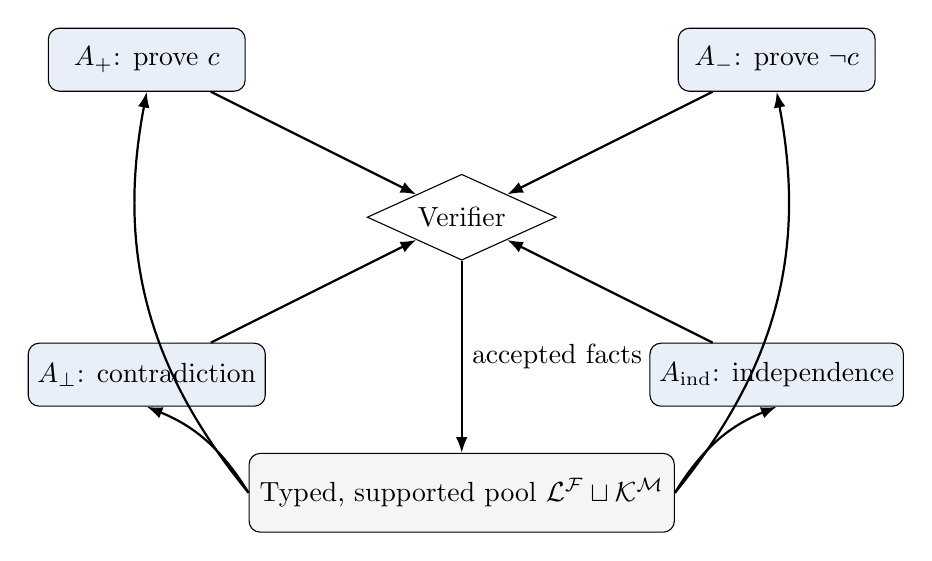
\begin{tikzpicture}[
  agent/.style={draw,rounded corners,minimum width=2.5cm,minimum height=0.8cm,fill=softblue},
  pool/.style={draw,rounded corners,minimum width=5.4cm,minimum height=1.0cm,fill=softgray},
  verify/.style={draw,diamond,aspect=2.2,fill=white},
  arr/.style={-{Latex[length=2mm]},thick}
]
\node[agent] (p) at (-4,2) {$A_{+}$: prove $c$};
\node[agent] (n) at (4,2) {$A_{-}$: prove $\neg c$};
\node[agent] (b) at (-4,-2) {$A_{\bot}$: contradiction};
\node[agent] (i) at (4,-2) {$A_{\mathrm{ind}}$: independence};
\node[verify] (v) at (0,0) {Verifier};
\node[pool] (l) at (0,-3.5) {Typed, supported pool $\Pool^{\F}\sqcup\MetaPool^{\M}$};
\draw[arr] (p) -- (v);
\draw[arr] (n) -- (v);
\draw[arr] (b) -- (v);
\draw[arr] (i) -- (v);
\draw[arr] (v) -- node[right]{accepted facts} (l);
\draw[arr] (l.west) to[bend left=25] (p.south);
\draw[arr] (l.east) to[bend right=25] (n.south);
\draw[arr] (l.west) to[bend right=18] (b.south);
\draw[arr] (l.east) to[bend left=18] (i.south);
\end{tikzpicture}
\caption{Every agent reads and writes through the verifier-controlled shared pool in every round.}
\end{figure}

\section{Machine-learned guidance as a later layer}

\subsection{What learning may control}
A learned policy may rank:
\begin{itemize}
  \item which agent receives the next expansion;
  \item which open goal or certificate obligation is selected;
  \item which inference, premise, model size, invariant template, or lemma is tried next;
  \item which verified pool lemmas are retrieved for a local state;
  \item whether a candidate lies just outside a deterministic cap and should receive counterfactual exploration.
\end{itemize}
Learning changes allocation of finite search effort. It does not change certificate acceptance.

\begin{theorem}[Verifier-separation theorem]
Fix sound certificate verifiers. Replace any deterministic or random ALD search policy by an arbitrary learned policy, even an adversarial one. Every accepted status remains sound.
\end{theorem}

\begin{proof}
The policy determines only which candidates are proposed and in what order. Acceptance is still determined by the unchanged sound verifier.
\end{proof}

\begin{definition}[Fairness-preserving learned policy]
Let $\pi_{\mathrm{ML}}$ be a learned scheduler and $\pi_0$ a fair baseline scheduler. A mixed policy is fairness-preserving if it reserves a recurrent positive share of search for $\pi_0$, for example
\[
\pi=(1-\varepsilon)\pi_{\mathrm{ML}}+\varepsilon\pi_0
\qquad(0<\varepsilon\le1),
\]
or uses a deterministic schedule that invokes $\pi_0$ infinitely often.
\end{definition}

\begin{theorem}[Fair guidance preserves certificate completeness]
If the baseline agent family is complete for a certificate class and the mixed scheduler is fairness-preserving, then learned guidance preserves eventual discovery of every certificate in that class.
\end{theorem}

\begin{proof}
The fair baseline receives infinitely many steps. Its complete enumeration therefore progresses without bound and eventually reaches any fixed finite certificate.
\end{proof}

\begin{remark}[Controlled creativity]
The exploration component has the same role as controlled counterfactual creativity in Predator 8.002: learning pulls useful actions toward the active frontier, while a protected exploration mechanism prevents an imperfect ranking from permanently excluding them.
\end{remark}

\subsection{Pool-aware learning}
The shared pool creates new learning targets. A lemma can be scored by cross-agent utility rather than only by whether it appeared in one final proof. Possible features include:
\begin{itemize}
  \item the number and diversity of agents that reused the lemma;
  \item reduction in open goals or model constraints after retrieval;
  \item proximity to a conclusive certificate;
  \item logical generality, proof cost, and dependency depth;
  \item whether the lemma bridged object and meta search through an explicitly checked interface.
\end{itemize}

A value model may estimate the probability that a global state will yield any conclusive certificate within the remaining budget. Separate heads may estimate $\Plus$, $\Minus$, $\BotEv$, and $\IndEv$ prospects. A meta-controller may allocate compute among agents while each local policy ranks its own actions.

\begin{protocol}[Leakage-controlled ALD training]
For a benchmark target $c$:
\begin{enumerate}[label=(\roman*)]
  \item freeze the formal database, checker, agent code, and certificate formats;
  \item exclude the target proof, target-specific independence proof, downstream results, and manually selected target routes from training;
  \item train only on earlier verified traces and earlier verified pool-use events;
  \item preserve a fair exploration channel;
  \item evaluate all statuses with independent fresh-process verification;
  \item report proof/certificate length, expansions, wall time, memory, status, and bounded unknown separately.
\end{enumerate}
\end{protocol}

\section{Examples of ALD settlement}

\subsection{Finite propositional logic}
For a finite propositional formula $c$ relative to finite assumptions $\Gammaa$, the proponent and opponent may use SAT proof search. A satisfying assignment for $\Gammaa\cup\{\neg c\}$ is a countermodel certificate showing $\Gammaa\nvdash c$; a satisfying assignment for $\Gammaa\cup\{c\}$ shows $\Gammaa\nvdash\neg c$. If both assignments exist, the model-pair theorem certifies independence. If one side is unsatisfiable, a checked LRAT-style refutation can certify derivability of the opposite side. Here an ALD can be total because the finite truth-assignment space is decidable.

\subsection{Finite algebra and first-order theories}
A theorem prover can search for a derivation while a finite model finder searches for a countermodel. A model does not refute the conjecture syntactically by itself; the model certificate plus semantic soundness proves nonderivability. Two models, one satisfying $c$ and one satisfying $\neg c$, yield independence when both are models of the same hypothesis theory.

\subsection{Set-theoretic independence}
For statements such as the Continuum Hypothesis, ordinary proof and refutation ATPs over ZFC are insufficient. The independence agent must search for or replay metatheoretic constructions showing, relative to an appropriate consistency assumption, a model of ZFC+$c$ and a model of ZFC+$\neg c$. The crucial computational event is not that two ZFC searches run forever. It is that a stronger formal environment checks two positive model or relative-consistency certificates.

\subsection{Predator-style ALD}
A Predator ALD can use four principal populations over a frozen Metamath environment:
\begin{itemize}
  \item one searches for the target theorem;
  \item one searches for its formal negation;
  \item one searches for an explicit contradiction or incompatible pair;
  \item one searches a metatheoretic library for saturation, invariant, model, interpretation, or relative-consistency certificates.
\end{itemize}
At every round, all populations read and write the verified lemma pool. The Metamath checker remains the object-level authority; a separate checker validates metatheoretic certificate forms. ML may guide all populations and pool retrieval, while the checker boundary remains unchanged.

\section{Further theory}

\subsection{Settlement depth vectors}
\begin{definition}[Status depth vector]
For a fixed ALD implementation and protocol define
\[
\mathbf d(\F,\Gammaa,c)=
(d_{+},d_{-},d_{\bot},d_{\mathrm{ind}}),
\]
where $d_e$ is the least global round at which an $e$-certificate is accepted, or $\infty$ if none is ever accepted.
\end{definition}

This vector retains more information than a single final status. It distinguishes a conjecture proved quickly but contradicted later from one proved quickly in a theory for which no inconsistency evidence is found.

\begin{proposition}[Contradiction depth bound]
Assume a fixed rule derives $\bottomf$ from $c$ and $\neg c$ in at most $k$ additional global expansions after both proofs are available. Then
\[
d_{\bot}\le \max(d_{+},d_{-})+k
\]
whenever both $d_{+}$ and $d_{-}$ are finite, unless a direct contradiction is found earlier.
\end{proposition}

\begin{proof}
At round $\max(d_+,d_-)$ both proof certificates are available in the pool. The contradiction agent can combine them using the fixed derivation within $k$ expansions.
\end{proof}

\subsection{Certificate transport under recoding}
\begin{theorem}[Recoding invariance of ALD status]
Let $t$ be an invertible syntactic recoding transporting $\F$, $\Gammaa$, $c$, proofs, models, and verifier inputs to a recoded instance. Assume every certificate verifier is equivariant under $t$. Then the original and recoded instances have the same accepted evidence types and the same logical status.
\end{theorem}

\begin{proof}
Transport accepted certificates forward with $t$ and backward with $t^{-1}$. Equivariance preserves acceptance, so each evidence type exists on one side exactly when it exists on the other.
\end{proof}

\begin{remark}
A recoding may change implementation cost if the parser, index, or learned features are presentation-sensitive, but it cannot change the certificate-defined status.
\end{remark}

\subsection{Settlement as a partially ordered evidence process}
The evidence ledger grows monotonically, but display statuses need not form a simple linear progression: $\Der$ can later become $\Both$, while $\Ind$ is incompatible with either under soundness. The more fundamental state is therefore the set $E_r$, ordered by inclusion. Logical settlement is an evidence accumulation process, and the display status is a projection of that richer state.

\begin{proposition}[Persistent evidence]
Once an evidence bit enters $E_r$, it remains in every $E_n$ for $n\ge r$.
\end{proposition}

\begin{proof}
The ledger update is by union.
\end{proof}

\begin{corollary}[Persistent certified claims]
A later search failure, timeout, or policy change cannot revoke an already accepted certificate. Revocation requires discovering that the verifier, frozen environment, or certificate was faulty, which is an audit event outside the formal run.
\end{corollary}

\subsection{Research conjectures}
\begin{conjecture}[Cross-status lemma advantage]
There are natural benchmark families for which a universally shared verified lemma pool yields an unbounded asymptotic reduction in settlement expansions over every architecture with role-isolated pools, even though both architectures use the same local ATP algorithms.
\end{conjecture}

\begin{conjecture}[Certificate-diversity advantage]
For some natural families, no single certificate method is efficient on all instances, while a fair ALD combining proof, refutation, model, invariant, and saturation agents has strictly better worst-case finite-budget coverage than any one constituent method.
\end{conjecture}

\begin{conjecture}[Learned pool utility transfer]
A leakage-controlled model trained to predict cross-agent lemma utility transfers better to unfamiliar theorem domains than a model trained only to predict membership in final proofs, because cross-agent reuse supplies a denser and more task-general supervision signal.
\end{conjecture}

\begin{conjecture}[ALD reflective ceiling]
For sufficiently expressive sound metatheories, there is no single internally verified ALD that both decides every object-theory sentence and fully certifies the soundness of all of its own status verifiers. Any practical hierarchy of ALDs therefore has a reflective ceiling or requires an external trust anchor.
\end{conjecture}

\section{Implementation blueprint}

\begin{lstlisting}[caption={Auditable round-synchronous ALD skeleton}]
input: frozen object theory F, hypotheses Gamma, conjecture c
initialize private agent states Q[i]
initialize provenance-aware typed pools L_object, L_meta
initialize evidence ledger E = empty

for round r = 1, 2, 3, ...:
    snapshot = (L_object, L_meta, E)

    proposals = parallel_for each agent i:
        return agent_step(i, Q[i], admissible_view(i, snapshot))

    for proposal p in deterministic_audit_order(proposals):
        if p.type == OBJECT_LEMMA and verify_object_with_support(p):
            L_object.add(p)
        elif p.type == META_LEMMA and verify_meta(p):
            L_meta.add(p)
        elif p.type in {PROOF_C, PROOF_NOT_C, PROOF_BOTTOM,
                        INDEPENDENCE_CERT} and verify_status(p):
            E.add(status_evidence_type(p))

    write_checkpoint(r, Q, L_object, L_meta, E)

    if frozen_halting_policy(Status(E)):
        emit(Status(E), accepted_certificates(E), audit_log)
        halt

    if frozen_resource_budget_exhausted():
        emit(UNKNOWN, budget_record, audit_log)
        halt
\end{lstlisting}

\subsection{Required audit record}
A reproducible ALD run should record:
\begin{itemize}
  \item hashes of the object theory, metatheory, checker binaries, agent code, and ML models;
  \item the conjecture, negation encoding, contradiction encoding, and hypotheses;
  \item the random seed and deterministic proposal-merge order;
  \item every accepted and rejected status certificate;
  \item every lemma-pool insertion, its logical level, assumption support, origin agent, proof certificate, support promotions, and first-use events;
  \item per-agent expansions, wall time, memory, and checkpoint state;
  \item the exact halting policy and resource budget;
  \item fresh-process verification of the final certificate bundle.
\end{itemize}

\section{Limitations and boundaries}

\begin{enumerate}[label=\textbf{L\arabic*.}]
  \item \textbf{Independence is metatheory-relative.} A certificate proves what $\M$ can soundly establish about $\F$.
  \item \textbf{No uniform totality.} Undecidability prevents a computable sound and complete ALD from settling every sentence of sufficiently expressive theories.
  \item \textbf{Model certificates may be unavailable or enormous.} Semantic existence does not imply a finite practical artifact.
  \item \textbf{Finite saturation requires true closure.} A fixed point inside an arbitrary truncated search space proves only bounded exhaustion, not global nonderivability.
  \item \textbf{Invariants are sufficient, not necessary.} Failure to find an invariant is $\Unknown$.
  \item \textbf{The pool can hurt performance.} Soundness survives irrelevant lemmas, but memory, provenance checks, and ranking can degrade; relevance filtering and support minimization are engineering necessities.
  \item \textbf{Learning does not certify.} It proposes and prioritizes; only the verifier licenses settlement.
  \item \textbf{A contradiction changes interpretation.} In an inconsistent object theory, deriving $c$ does not exclude deriving $\neg c$. The evidence ledger is more informative than a single truth-like label.
\end{enumerate}

\section{Conclusion}
The central problem of computer-detected independence is not solved by waiting for two proof searches to fail. It is solved, when it is solvable, by searching for positive certificates that both derivations are impossible. A multiagent ALD turns this into an explicit architecture: proof, negation-proof, inconsistency, and independence roles run concurrently; every agent can add to and inspect a shared verified lemma pool in every round; object and meta records remain distinct; and assumption provenance prevents a branch theorem from being mistaken for a theorem of the base theory. Finite saturation, invariants, model pairs, relative consistency, and formal metaproofs become first-class halting mechanisms. Timeouts remain bounded unknown. Machine learning may later allocate search attention and predict cross-agent lemma utility without weakening soundness, provided certificate checking, provenance enforcement, and fairness remain outside the learned component.

The literature already contains cooperative provers, blackboard systems, lemma exchange, model-based non-theorem statuses, the SZS \emph{NoConsequence} relation, formal independence proofs, and learned proof guidance. The research opportunity is therefore not to claim those pieces individually. It is to develop and test their unified certificate-indexed theory: a SIC-style ALD with a monotone evidence ledger and a universally visible, provenance-aware lemma pool. Undecidability prevents this from becoming a universal total decision procedure, but it does not prevent many formerly silent non-halting cases from becoming finitely, positively, and audibly settled.

\clearpage
\section*{References and research context}
\addcontentsline{toc}{section}{References and research context}
\begin{thebibliography}{99}

\bibitem{SZS}
G. Sutcliffe,
``The SZS Ontologies and Presentation Standards,''
TPTP World documentation, including the \emph{NoConsequence} status and proof/model data forms,
accessed August 2, 2026.

\bibitem{BonacinaHsiang1995}
M. P. Bonacina and J. Hsiang,
``The Clause-Diffusion Methodology for Distributed Deduction,''
\emph{Fundamenta Informaticae}, 24(1--2):177--207, 1995.
DOI: 10.3233/FI-1995-24128.

\bibitem{DenzingerKronenburgSchulz1997}
J. Denzinger, M. Kronenburg, and S. Schulz,
``DISCOUNT---A Distributed and Learning Equational Prover,''
\emph{Journal of Automated Reasoning}, 18(2):189--198, 1997.
DOI: 10.1023/A:1005879229581.

\bibitem{Fuchs1998}
D. Fuchs,
``Requirement-Based Cooperative Theorem Proving,''
in \emph{Logics in Artificial Intelligence: JELIA '98}, LNAI 1489, pp. 139--153, Springer, 1998.

\bibitem{LeoII}
C. Benzm\"uller, N. Sultana, L. C. Paulson, and F. Thei\ss,
``The Higher-Order Prover Leo-II,''
\emph{Journal of Automated Reasoning}, 55:389--404, 2015.
DOI: 10.1007/s10817-015-9348-y.

\bibitem{WisniewskiBenzmuller2016}
M. Wisniewski and C. Benzm\"uller,
``Is It Reasonable to Employ Agents in Automated Theorem Proving?''
in \emph{Proceedings of ICAART 2016}, vol. 1, pp. 281--286.
DOI: 10.5220/0005824702810286.

\bibitem{Kim2016}
D. Kim,
``Distributed Agent-Based Automated Theorem Proving in Order-Sorted First-Order Logic,''
\emph{arXiv:1609.02320}, 2016.

\bibitem{HarrisonThery1998}
J. Harrison and L. Th\'ery,
``A Skeptic's Approach to Combining HOL and Maple,''
\emph{Journal of Automated Reasoning}, 21:279--294, 1998.
DOI: 10.1023/A:1006023127567.

\bibitem{McCune2003}
W. McCune,
``Mace4 Reference Manual and Guide,''
\emph{arXiv:cs/0310055}, 2003.

\bibitem{RegerSudaVoronkov2016}
G. Reger, M. Suda, and A. Voronkov,
``Finding Finite Models in Multi-Sorted First-Order Logic,''
\emph{arXiv:1604.08040}, 2016.

\bibitem{HanVanDoorn2021}
J. M. Han and F. van Doorn,
``A Formal Proof of the Independence of the Continuum Hypothesis,''
\emph{arXiv:2102.02901}, 2021.

\bibitem{KaliszykUrban2015}
C. Kaliszyk and J. Urban,
``Learning-Assisted Theorem Proving with Millions of Lemmas,''
\emph{Journal of Symbolic Computation}, 69:109--128, 2015.
DOI: 10.1016/j.jsc.2014.09.032.

\bibitem{KaliszykUrbanVyskocil2015}
C. Kaliszyk, J. Urban, and J. Vysko\v{c}il,
``Lemmatization for Stronger Reasoning in Large Theories,''
in \emph{FroCoS 2015}, LNAI 9322, pp. 341--356.
DOI: 10.1007/978-3-319-24246-0\_21.

\bibitem{JakubuvUrban2017}
J. Jakub\r{u}v and J. Urban,
``ENIGMA: Efficient Learning-Based Inference Guiding Machine,''
\emph{arXiv:1701.06532}, 2017.

\bibitem{ProverAgent2025}
K. Baba, C. Liu, S. Kurita, and A. Sannai,
``Prover Agent: An Agent-Based Framework for Formal Mathematical Proofs,''
\emph{arXiv:2506.19923}, 2025.

\bibitem{AgentHunt2026}
C. E. Brown, C. Kaliszyk, and J. Urban,
``Agent Hunt: Bounty Based Collaborative Autoformalization With LLM Agents,''
\emph{arXiv:2603.06737}, 2026.

\end{thebibliography}

\end{document}
